%!TEX program = xelatex
% Note: this template must be compiled with XeLaTeX rather than PDFLaTeX
% due to the custom fonts used. The line above should ensure this happens
% automatically, but if it doesn't, your LaTeX editor should have a simple toggle
% to switch to using XeLaTeX.

\documentclass[
  aspectratio=169, % Uncomment to use an aspect ratio of 16:9 (160 mm by 90 mm)
  %aspectratio=43, % Uncomment to use an aspect ratio of 4:3 (128mm by 96mm)
  t, % Top align all slide content by default
  onlytextwidth, % Typeset content in columns at text width
  10pt, % Default font size, use 10pt for the 16:9 aspect ratio and 8pt for the 4:3 aspect ratio
]{beamer}

\usepackage{../../ImperialTheme/beamer/beamerthemeImperial} % Use the Imperial theme
\usepackage{tikz}
\usetikzlibrary{calc}


\def\imagefolder{../../ImperialTheme/beamer/Images}
\def\Rey{\text{Re}}
\title{Stability diagram} % Presentation title to appear on the title slide and left footers

\subtitle{} % Presentation subtitle to appear on the title slide

\author{Víctor Ballester} % Author name(s) to appear on the title slide

\date{\today} % Presentation date to appear on the title slide and right footers

\begin{document}

\begingroup
\setbeamercolor{background canvas}{bg=ICLLightGrey} % Slide background color
\setbeamercolor{title page title}{fg=ICLBlue} % Title text color
\setbeamercolor{title page subtitle}{fg=ICLBlue} % Subtitle text color
\setbeamercolor{author}{fg=ICLBlue} % Author(s) text color
\setbeamercolor{date}{fg=ICLBlue} % Date text color
\setbeamertemplate{title page}[logo]{\imagefolder/ICL_Logo_Blue.pdf} % Imperial logo color, use 'ICL_Logo_White.pdf' for white and 'ICL_Logo_Blue.pdf' for blue
\frame[plain, s]{\titlepage} % Output the title page with no footer ('plain') and vertically distributed text ('s')
\endgroup

\begin{frame}
	\frametitle{Stability diagram}
	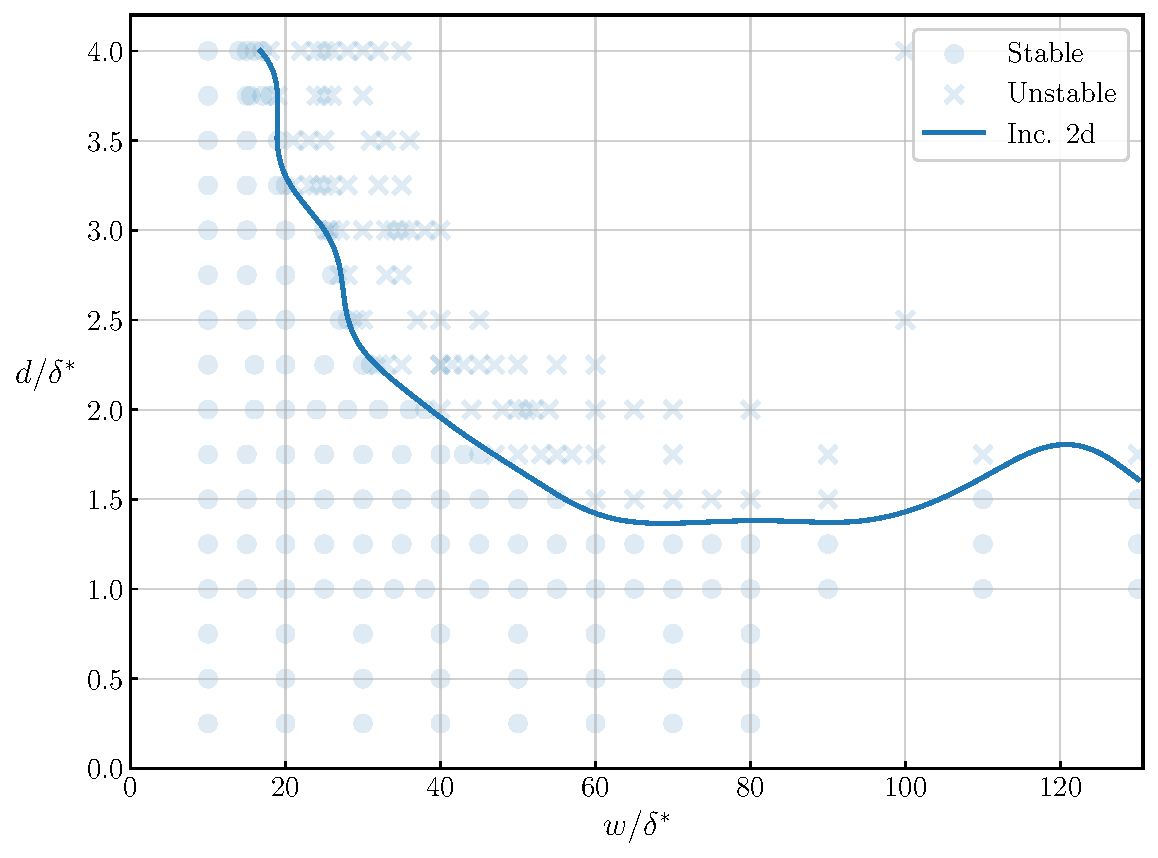
\includegraphics[width=0.65\linewidth]{../../../images/stabilityCurve.pdf}
\end{frame}
\begin{frame}
	\frametitle{Sponge region}

	\begin{itemize}
		\item With and without sponge region ($d=3$, $w=15$). Top and outflow boundary conditions. Inflow no (so far) because of stability issues (bad resolution of the boundary layer with p=1 near the BC)
	\end{itemize}
	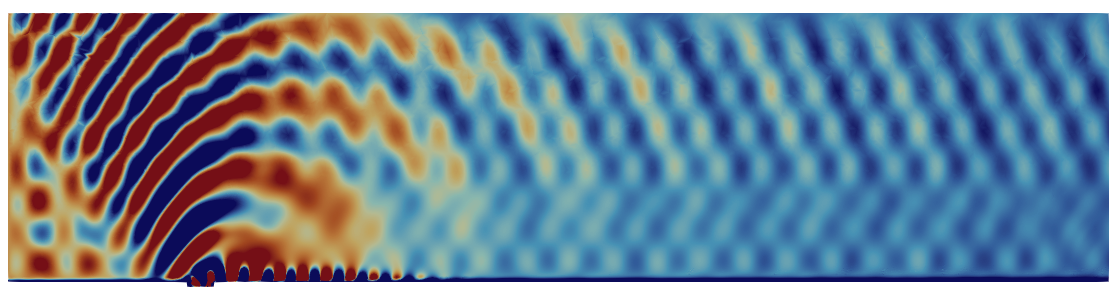
\includegraphics[width=0.75\linewidth]{Images/d3_w15_nosponge.png}
	\begin{tikzpicture}
		\node[inner sep=0] (img) {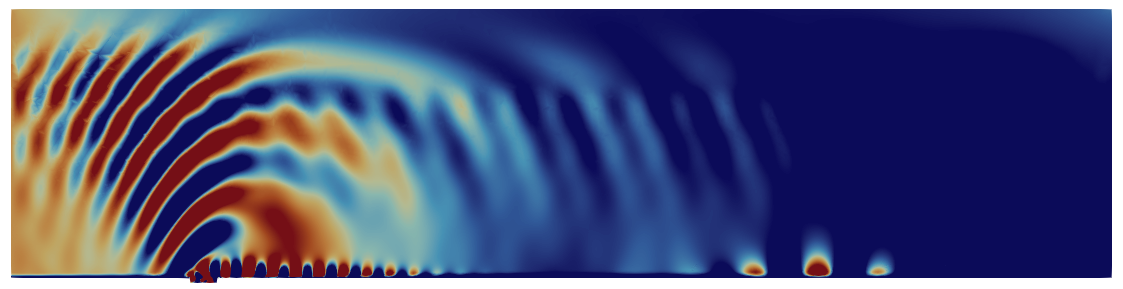
\includegraphics[width=0.75\linewidth]{Images/d3_w15_sponge.png}}; % replace with your file
		% Draw a rectangle border (no fill) around some region of the image.
		% Coordinates relative to the image node anchors:
		% (img.north west), (img.south east), etc. We shift the corners to get the square we want.
		\draw[line width=1.5pt, red]
		($(img.north west)+(0.01\textwidth,-0.007\textwidth)$) rectangle
		($(img.south east)+(-0.007\textwidth,0)+0.66666*(img.north east) - 0.66666*(img.south east)$);

		\draw[line width=1.5pt, green!70!black]
		($(img.north east)+(0,-0.007\textwidth)-0.0813*(img.north east) + 0.0813*(img.north west)$) rectangle
		($(img.south east)+(-0.007\textwidth,0.01\textwidth)$);

	\end{tikzpicture}
\end{frame}
\begin{frame}
  \frametitle{2nd bif Inc}
  \begin{itemize}
    \item Most energetic frequency as function of $w$ (in the linearly unstable regime).
  \end{itemize}
  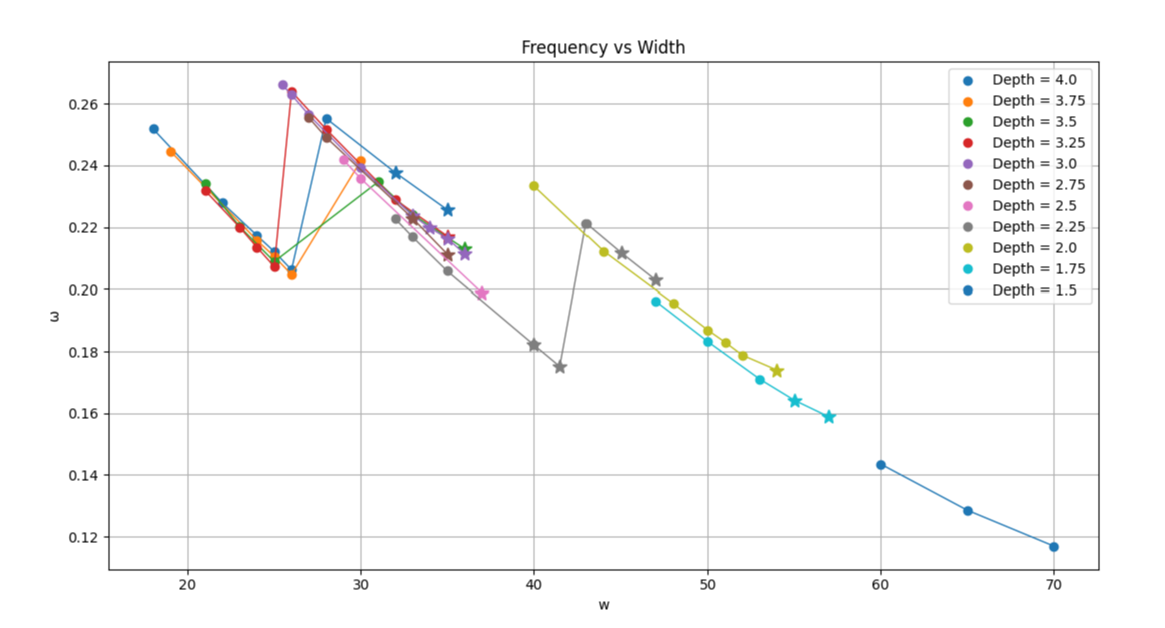
\includegraphics[width=0.85\linewidth]{Images/freqs.png}  

\end{frame}
\begin{frame}
  \frametitle{Example of $d=1.75$ - 1}
  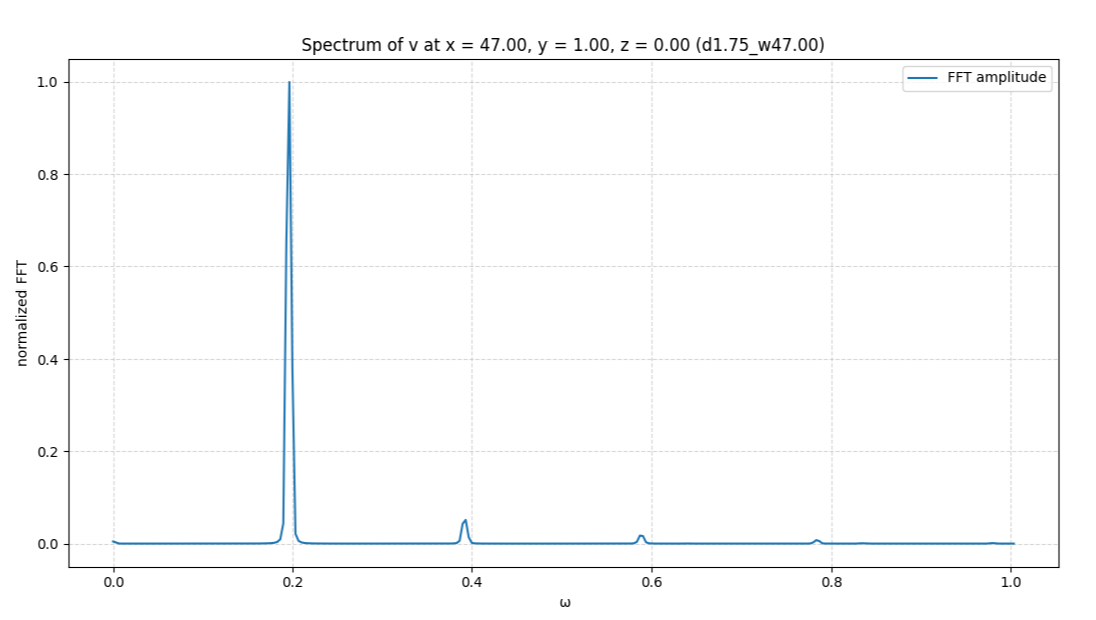
\includegraphics[width=0.85\linewidth]{Images/d1.75_w47_freq.png}
  
\end{frame}
\begin{frame}
  \frametitle{Example of $d=1.75$ - 2}

  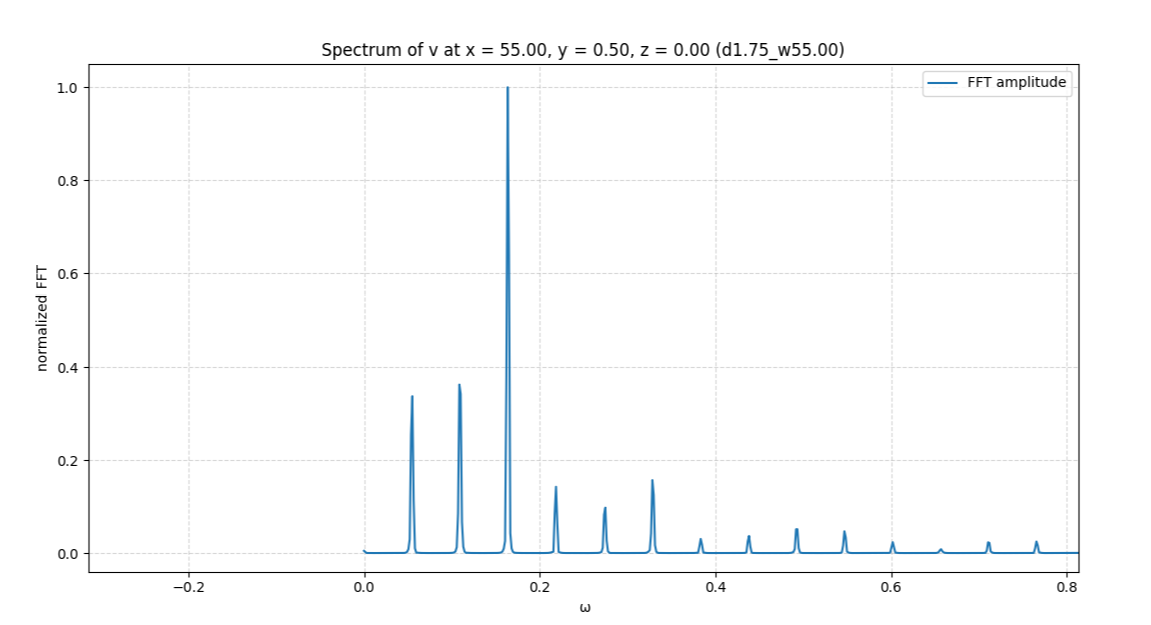
\includegraphics[width=0.85\linewidth]{Images/d1.75_w55_freq.png}
  
\end{frame}
\begin{frame}
  \frametitle{Example of $d=1.75$ - 3}
  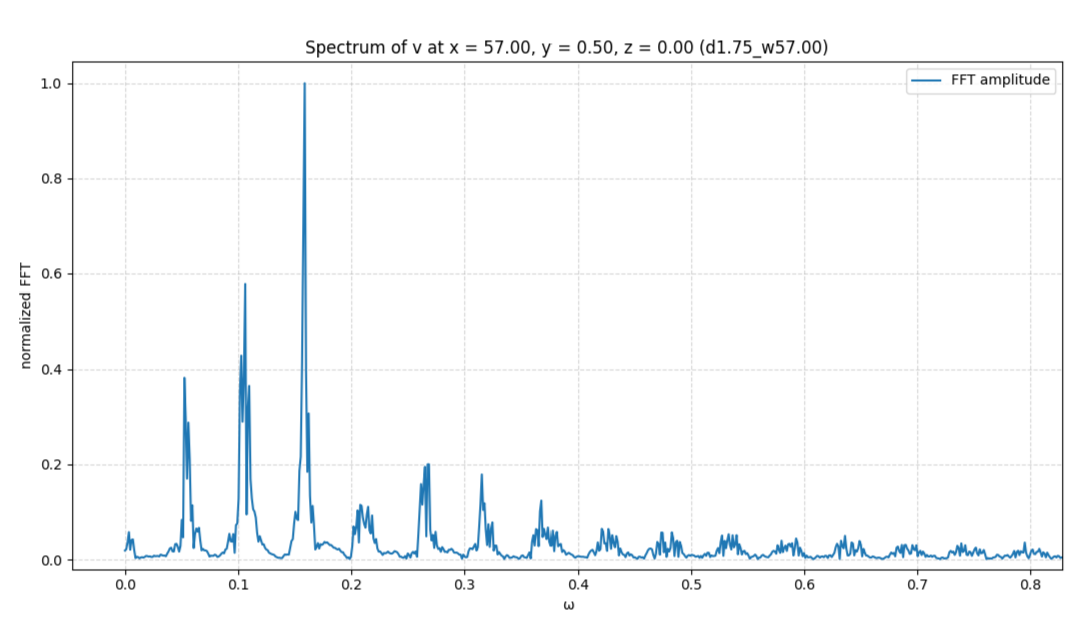
\includegraphics[width=0.85\linewidth]{Images/d1.75_w57_freq.png}
  
\end{frame}
\begin{frame}
  \frametitle{Example of $d=2.25$ - 1}
  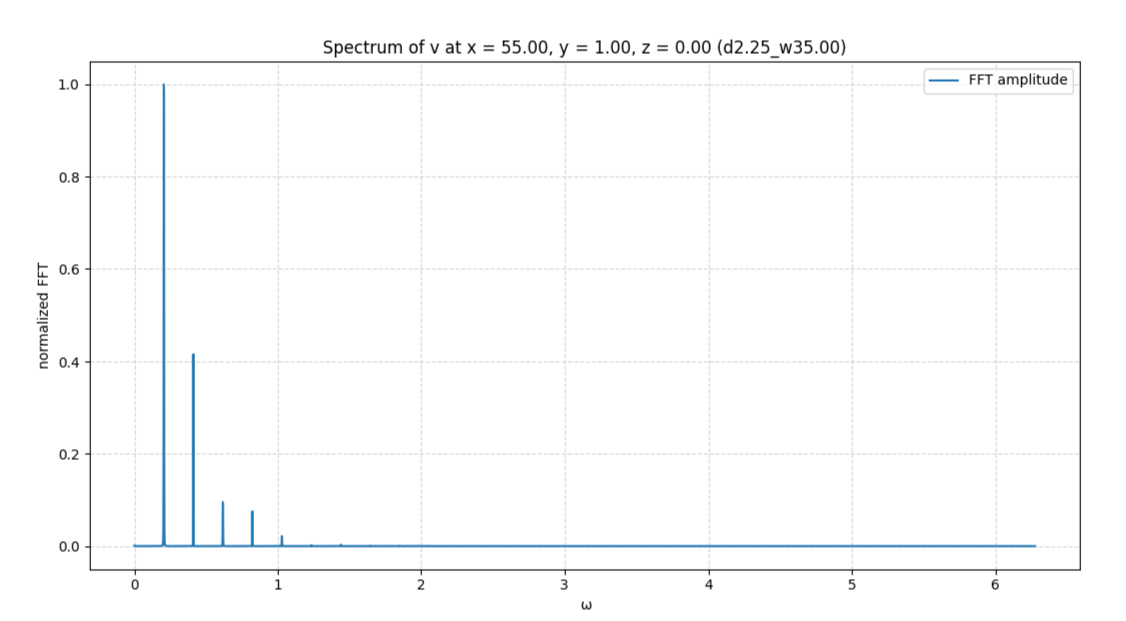
\includegraphics[width=0.85\linewidth]{Images/d2.25_w35_freq.png}
  
\end{frame}
\begin{frame}
  \frametitle{Example of $d=2.25$ - 1}
  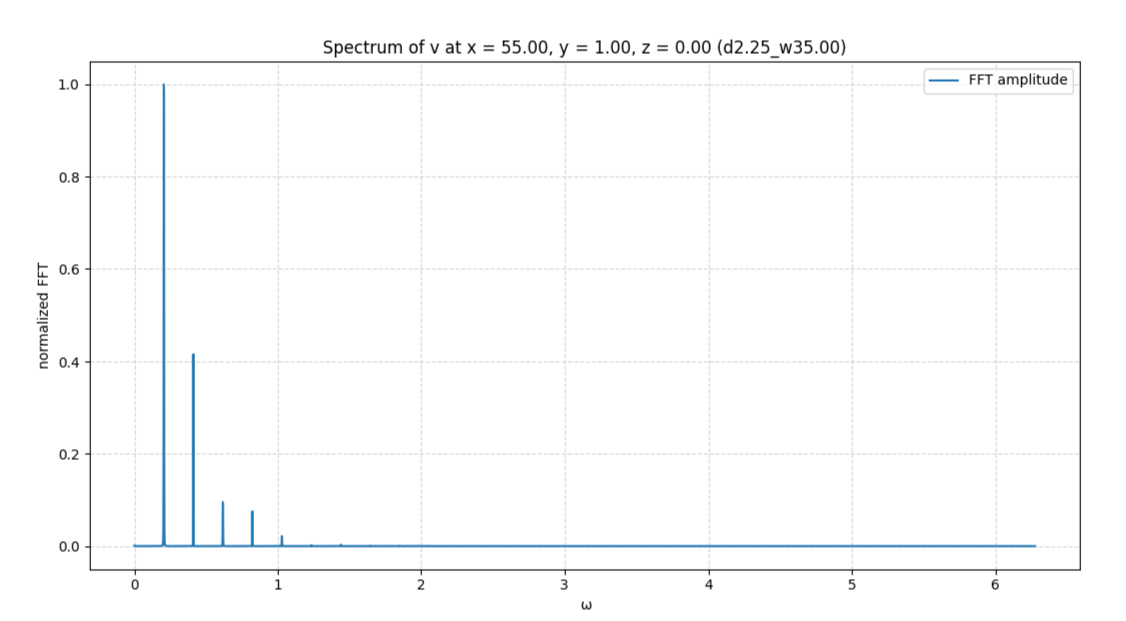
\includegraphics[width=0.85\linewidth]{Images/d2.25_w35_freq.png}
  
\end{frame}
\begin{frame}
  \frametitle{Example of $d=2.25$ - 2}
  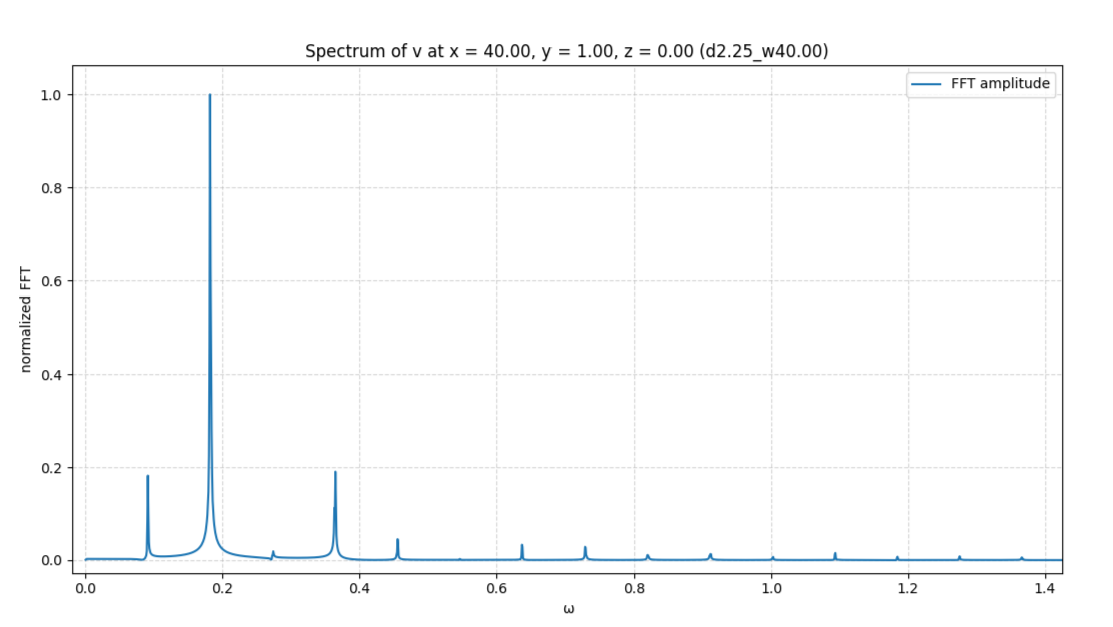
\includegraphics[width=0.85\linewidth]{Images/d2.25_w40_freq.png}
  
\end{frame}
\begin{frame}
  \frametitle{Example of $d=2.25$ - 3}
  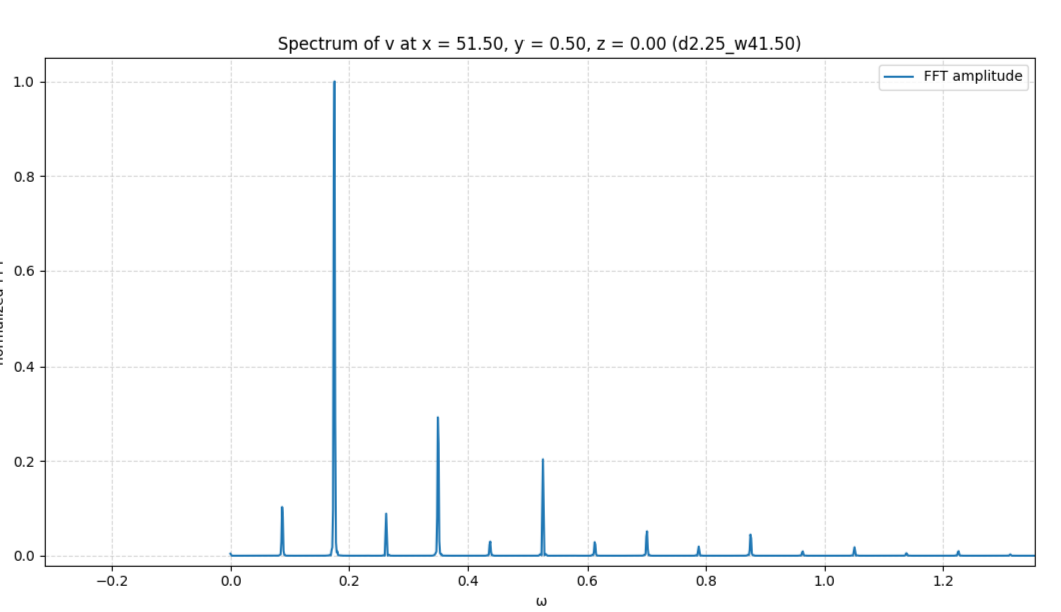
\includegraphics[width=0.85\linewidth]{Images/d2.25_w41.5_freq.png}
  
\end{frame}
\begin{frame}
  \frametitle{Example of $d=2.25$ - 4}
  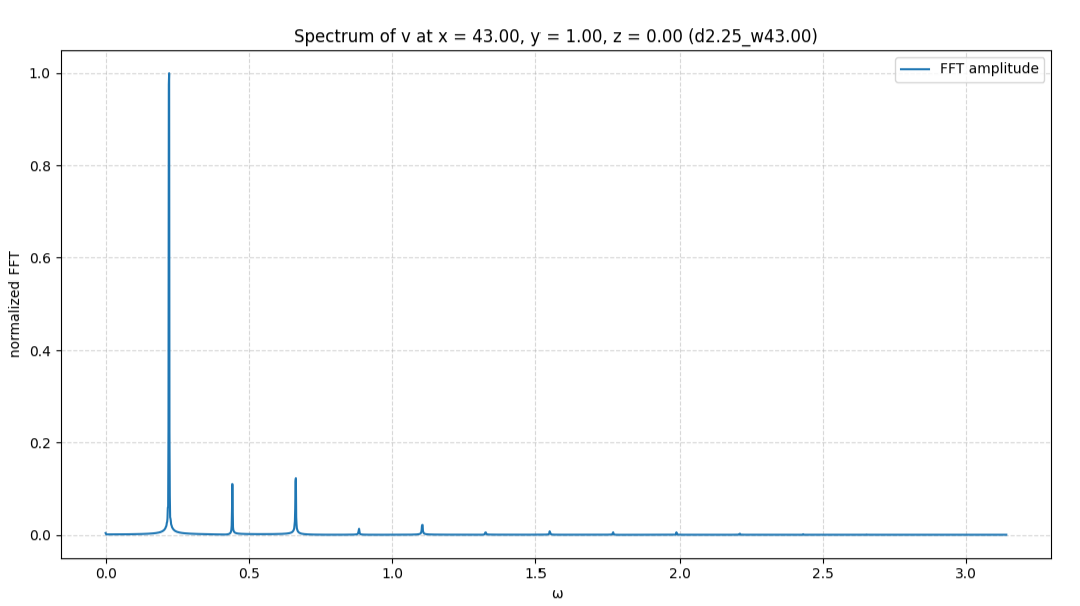
\includegraphics[width=0.85\linewidth]{Images/d2.25_w43_freq.png}
  
\end{frame}
\begin{frame}
  \frametitle{Example of $d=2.25$ - 5}
  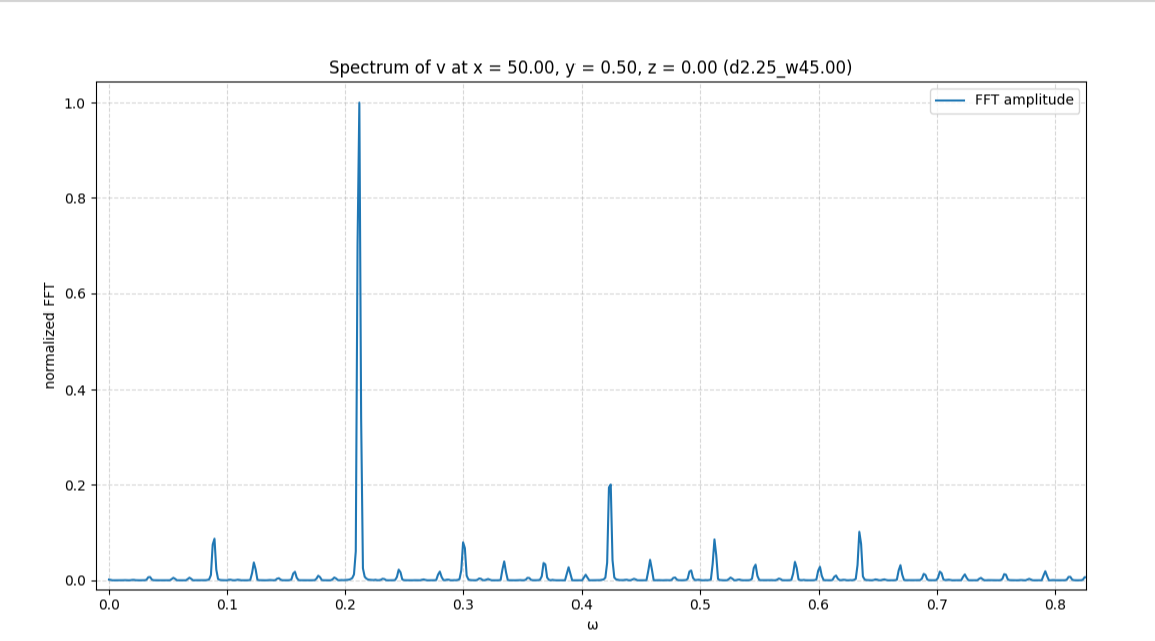
\includegraphics[width=0.85\linewidth]{Images/d2.25_w45_freq.png}
  
\end{frame}
\end{document}
